\section{Linee guida per gli esercizi}
\subsection{Impostazione del problem}
\begin{itemize}
    \item Leggere bene il testo del problema.
    \item Effettuare una schematizzazione del problema: identificare il tipo di sistema, il suo
    contorno, la sostanza evolvente nel sistema, gli scambi di massa, calore e lavoro con
    l’ambiente e la loro direzione.
    \item Scrivere i dati forniti dal testo del problema, e le incognite da ricavare per risolverlo.
    Convertire i dati in unità di misura congruenti e conformi al Sistema Internazionale.
    \item Se avvengono trasformazioni termodinamiche, rappresentarle qualitativamente su un
    diagramma opportuno.    
\end{itemize}
\subsection{Soluzione del problema}
\begin{itemize}
    \item Scrivere i bilanci di massa, energia ed entropia per il volume di controllo considerato.
    Elencare le ipotesi applicabili al sistema (riguardo la natura del contorno del sistema, delle
    trasformazioni che avvengono al suo interno, delle sostanze delle quali è composto), e
    semplificare i bilanci di conseguenza, ponendo attenzione alle convenzioni di segno.
    \item Scrivere la soluzione analitica del problema.
    \item Risolvere il problema numericamente. Si raccomanda di scrivere sempre le unità di misura
    delle grandezze calcolate e di fare l’analisi dimensionale delle equazioni scritte.
    \item Fare sempre caso alla ragionevolezza dei risultati  
\end{itemize}
\subsection{Unità di misura}
\begin{center}
    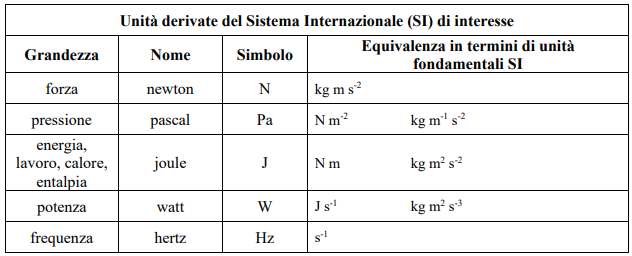
\includegraphics[height=5cm]{../L01/img10.PNG}
\end{center}
\begin{center}
    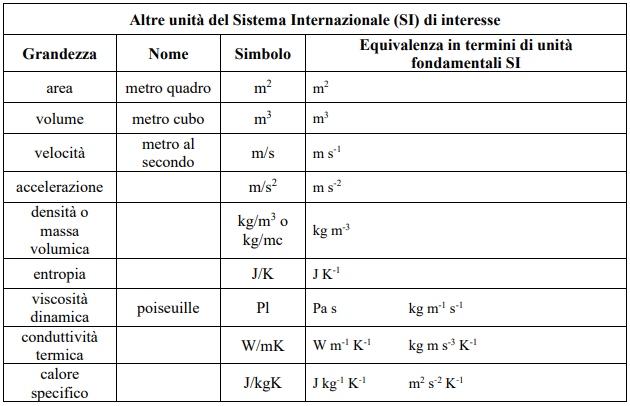
\includegraphics[height=7cm]{../L01/img11.PNG}
\end{center}
\begin{center}
    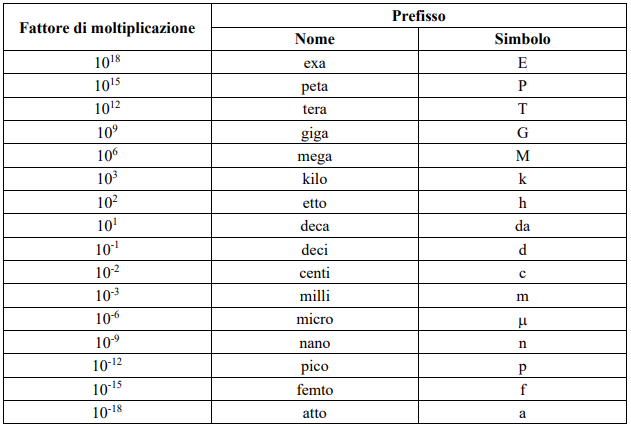
\includegraphics[height=5cm]{../L01/img12.PNG}
\end{center}
\begin{center}
    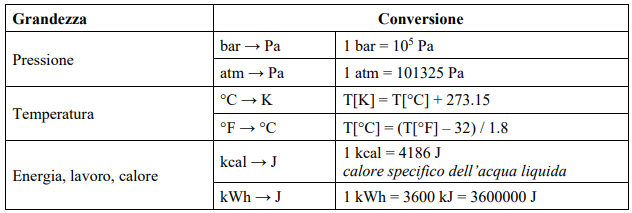
\includegraphics[height=5cm]{../L01/img13.PNG}
\end{center}
\section{Equazioni di bilancio per i sistemi chiusi}
Un \textbf{sistema chiuso} è un sistema per il quale non sono consentiti scambi di massa attraverso il suo contorno. Per tale sistema non è in uso applicare \textbf{equazioni di bilancio di massa} essendo implicita la sua conservazione nella definizione di sistema chiuso.\newline
\newline
Nelle soluzioni di problemi con sistemi chiusi le equazioni fondamentali sono \textbf{l'equazione di bilancio energetico} e \textbf{l'equazione di bilancio entropico} che assumono la forma:
\[
    \Delta U = Q^\leftarrow  -L^\rightarrow  
\]
\[
    \Delta S = S_Q + S_{irr}
\]
cioè la variazione di energia interna è pari alla differenza tra il calore entrante nel sistema e il lavoro ceduto dal sistema; la variazione di entropia è pari alla somma della entropia $S_Q$ entrante attraverso il contorno del sistema con il calore Q e della quantità $S_{irr}$ generata all'interno del sistema per irreversibilità. Questa ultima quantità è sempre positiva e tende a zero col tendere dei processi alla reversibilità. Inoltre il segno del termine $S_Q$ è sempre uguale al segno di $Q$.\newline
\newline
L'\textbf{energia interna} e l'\textbf{entropia} sono proprietà \textbf{estensive e additive}. Quindi dato un sistema $Z$ composto da due sottosistemi $A$ e $B$, posso scrivere:
\[
    \Delta U_Z = \Delta U_A + \Delta U_B = Q_Z^\leftarrow  - L_Z^\rightarrow  \;\;\;\;\;\;\;\;\;\;\Delta S_Z = \Delta S_A + \Delta S_B = S_{Q,Z} + S_{irr,Z}
\]
\ \newline
\newline
Se il \textbf{lavoro scambiato} è lavoro meccanico quasi-statico (internamente reversibile), è determinabile con l'espressione:
\[
    L = \int_{i}^{f} P dV
\]
Questa espressione è integrabile se è nota l'equazione della trasformazione ovvero la funzione:
\[
    P = P(V)
\]
\ \newline
Il \textbf{calore scambiato}, nell'ipotesi di trasformazione quasi-statica, può essere determinato avendo noto il calore specifico della trasformazione:
\[
    Q = M c_x (T_2-T_1)
\]
\ \newline
L'\textbf{energia interna} di un sistema in uno stato di equilibrio può essere espressa in funzione di altre proprietà intensive ed estensive specifiche del sistema come la temperatura, il volume specifico, la pressione. Particolarmente utili sono i due seguenti casi in cui è possibile esprimere in una forma analitica elementare il legame funzionale tra la variazione di energia interna tra due stati di equilibrio e la variazione di temperatura. \newline
\textbf{Gas perfetto}: $\Delta u = c_V (T_2 - T_1)$\newline
\textbf{Liquido incomprimibile perfetto}: $\Delta u = c(T_2-T_1)$\newline
Inoltre:
\begin{itemize}
    \item Per un sistema isolato $\Delta U_{isolato} = 0$.
    \item Per un sistema che subisce una trasformazione ciclica: $\Delta U_{ciclo} = 0$
\end{itemize}
\ \newline
\newline
Il caso di trasformazioni quasi-statiche a pressione costante o trasformazioni irreversibili in un sistema con stato iniziale e finale alla stessa pressione consente di scrivere l’equazione di bilancio energetico per il sistema chiuso come:
\[
    \Delta H = Q \;\;\;\;\;\;\;\;\;\;\;\;\;\;\;\text{dove $h = u + Pv$}\;
\]
Per esempio la miscelazione adiabatica e isobara di due sottosistemi produce uno stato finale caratterizzato da un valore di entalpia totale pari alla somma delle entalpia iniziale dei due sottosistemi. \newline
L'\textbf{entalpia specifica} di un sistema in uno stato di equilibrio può essere espressa
in funzione di altre proprietà intensive ed estensive specifiche del sistema come la
temperatura, il volume specifico, la pressione. Particolarmente utili sono i due seguenti casi
in cui è possibile esprimere in una forma analitica elementare il legame funzionale tra la
variazione di entalpia specifica tra due stati di equilibrio e la variazione di temperatura. \newline
\textbf{Gas perfetto}: $\Delta h = c_P (T_2 - T_1)$\newline
\textbf{Liquido incomprimibile perfetto}: $\Delta h = c(T_2-T_1) + v(P_2-P_1)$\newline
\newline
L'\textbf{entropia} è una proprietà del sistema e quindi dipende solo dallo stato del sistema: ne consegue che noti gli stati iniziale e finale di un processo, la determinazione della variazione di entropia prescinde dalla conoscenza di qualsiasi dettaglio del processo (ivi compresa la sua reversibilità). Particolarmente utili sono i due seguenti casi in cui è possibile esprimere in una forma analitica elementare il legame funzionale tra l'entropia e altre proprietà del sistema. Per il gas perfetto sono possibili 3 diverse espressioni che fanno uso di 3 diverse coppie di coordinate termodinamiche indipendenti. \newline
\textbf{Gas perfetto}:
\[
    \begin{matrix}
        \Delta s = c_P ln \frac{T_2}{T_1} - R^* ln \frac{P_2}{P_1} \;\;\;\;\;\;\;\;\;\;\;\;\;\;\;\Delta s = c_V ln \frac{T_2}{T_1} + R^* ln \frac{V_2}{V_1}\\
        \Delta s = c_V ln \frac{P_2}{P_1} + c_P ln \frac{V_2}{V_1}
    \end{matrix}
\]
\textbf{Liquido incomprimibile perfetto}: $\Delta s = c ln \frac{T_2}{T_1}$\newline
Inoltre:
\begin{itemize}
    \item Per definizione la variazione di entropia di un serbatoio di lavoro ($\Delta S_{SL}$) è nulla.
    \item Per definizione la variazione di entropia di un serbatoio di calore ($\Delta S_{SC}$) ha solo la componente reversibile, gli scambi avvengono con trasformazioni quasi-statiche (internamente reversibili).
    \item Un processo è impossibile da realizzare nel momento in cui $S_{irr} < 0$.
    \item La variazione di entrpia per una trasformazione reversibile è data da $\Delta S = \int_{i}^f \frac{1}{T} \delta Q_{rev}^\leftarrow$ (per i casi in cui $T$ è costante, allora $\Delta S = \frac{Q}{T}$).
    \item La variazione di entropia totale di un sistema isolato sede di trasformazioni termodinamiche è
    sempre maggiore di zero e tende a zero con il tendere dei processi alla reversibilità $\Delta S_{isolato} \geq 0$.
    \item $S_{irr} \geq 0$ è sempre maggiore di zero e il segno di $S_{Q}^\leftarrow $ è uguale al segno di $Q^\leftarrow$
\end{itemize}
\ \newline
\newline
\textbf{L’energia interna, l’entalpia e l’entropia} sono proprietà del sistema e quindi dipendono solo
dallo stato del sistema: ne consegue che noti gli stati iniziale e finale di un processo, la
determinazione della loro variazione prescinde dalla conoscenza di qualsiasi dettaglio del
processo (ivi compresa la sua reversibilità). Non è invece possibile determinare \textbf{il lavoro ed il
calore} scambiato dal sistema nel caso in cui si conoscano solo stato iniziale e finale e in tal caso non si ricorre pertanto alla scrittura del bilancio di energia (primo principio) e di entropia (secondo principio) che risulterebbero
indeterminati, ma si ricorre alle equazioni di stato (per i gas perfetti o per i liquidi incomprimibili perfetti\dots) che utilizzano solamente dati dello stato iniziale e finale.
\section{Stati monofase: equazioni di stato e trasformazioni}
Le sostanze nello stato monofase possono schematicamente essere suddivise in sostanze nello
stato aeriforme, liquido o solido. I modelli di equazioni di stato sono, in prima
approssimazione, ricondotti a modelli ideali o modelli reali.
\subsection{Gas ideali}
Le equazioni di stato dei \textbf{gas ideali} sono:
\[
    PV=MR^*T
\]
\[
    U=U(T) \;\;\;\;\;\;\;\;\;\;\;\;\Delta U = M c_V \Delta T \rightarrow \Delta u = c_V \Delta T
\]
La costante $R^*$ rappresenta la costante del gas ed è determinabile con la relazione:
\[
    R^* = \frac{R}{M_m}
\]
\[
    R=8314 [J/kmole K] =\text{costatne universale dei gas}\; \;\;\;\;\;\;\;\;\;\;M_m = \text{massa molare}\;
\]
\begin{center}
    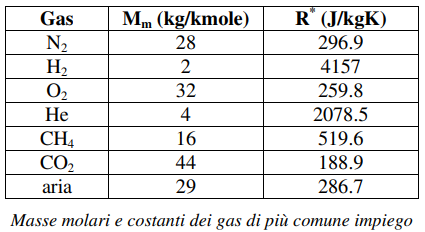
\includegraphics[height=3cm]{../NOTE SUGLI ESERCIZI/img1.PNG}
\end{center}
La grandezza $c_V$ rappresenta il calore specifico a volume costante funzione del gas e della sua
struttura molecolare. Qualora il calore specifico a volume costante possa assumersi indipendente dalla temperatura (e quindi costante) si parla di gas perfetto.
\subsection{Liquidi e solidi incomprimibili ideali}
Le equazioni di stato dei fluidi incomprimibili ideali (liquidi e solidi) sono:
\[
    v = costante
\]
\[
    U=U(T)  \;\;\;\;\;\;\;\;\;\;\;\;\Delta U = M c \Delta T \rightarrow \Delta u = c \Delta T
\]
dove $c$ è il calore specifico della sostanza.
\subsection{Gas reali}
Una possibile equazione di stato dei gas reali è:
\[
    Pv = ZRT
\]
dove $Z$ è il fattore di compressibilità. Tale coefficiente è determinabile attraverso il diagramma generalizzato che riposta il fattore di compressibilità in funzione della pressione e della temperatura ridotta. La pressione e la temperatura ridotte sono valori adimensionali ottenuti dalle relazioni:
\[
    P_R = \frac{P}{P_{cr}} \;\;\;\;\;\;\;\;\;\;\;\;\;\;\;T_R = \frac{T}{T_{cr}}
\]
in cui $P_{cr}$ e $T_{cr}$ rappresentano i valori di pressione e temperatura nello stato critico.
\begin{center}
    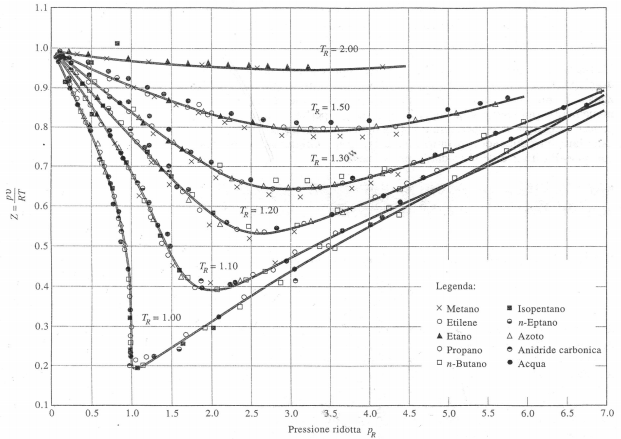
\includegraphics[height=5cm]{../NOTE SUGLI ESERCIZI/img2.PNG}
\end{center}
\subsection{Liquidi e solidi reali}
Le equazioni di stato dei liquidi e solidi reali sono formulate in forma differenziale:
\[
    dv = \beta v \cdot dT - K_Tv \cdot  dP
\]
\[
    \text{Coefficiente di dilatazione termica isobaro}\;\;\;\beta = \frac{1}{v} \left(\frac{\delta v}{\delta T}\right)_P
\]
\[
    \text{Coefficiente di comprimibilità isotermo}\;\;\;K_T = - \frac{1}{v} \left(\frac{\delta v}{\delta P}\right)_T
\]
Siccome $\beta$ e $K_T$ possono essere considerati costanti per ampi intervalli di temperatura e di pressione, la precedente relazione differenziale è integrabile e lo stato calcolabile.
\begin{center}
    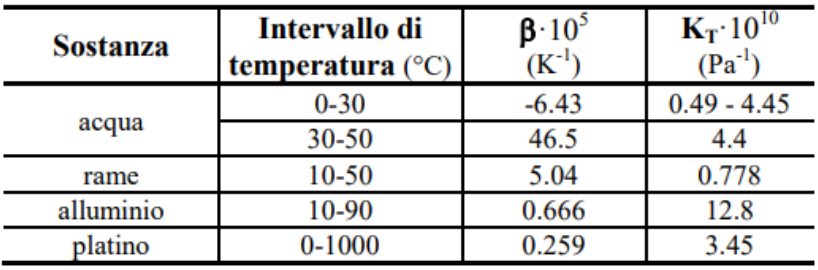
\includegraphics[height=3cm]{../NOTE SUGLI ESERCIZI/img3.PNG}
\end{center}
\subsection{Trasformazioni politropiche}
Le \textbf{trasformazioni politropiche} sono trasformazioni termodinamiche \textbf{internamente reversibili}
proprie dei \textbf{gas perfetti} e caratterizzate dall’avere un calore specifico $c_x$ \textbf{costante}.\newline
\newline
L’equazione della politropica in coordinate P,v risulta
\[
    Pv^n = costante \;\;\;\;\;\;\;\;\;\;\text{dove \textbf{l'indice della politropica} è}\;\;\;n = \frac{c_x - c_P}{c_x - c_V}
\]
Con l’ausilio dell’equazione di stato dei gas ideali è possibile ottenere espressioni
dell’equazione della politropica in coordinate T,P e T,v: 
\[
    P^{1-n}T^n = costante
\]
\[
    Tv^{n-1} = costante
\]
Si distinguono alcune trasformazioni elementari particolarmente utili tra le politropiche: 
\begin{center}
    \begin{tabular}{ |c|c|c|c| } 
        \hline
        Trasformazione & $c_x$ & $n = \frac{c_x - x_P}{c_x - c_V}$ \\
        \hline
        Isoterma ($T = costante$) & $\pm \infty$ & $1$ \\ 
        Isocora ($v = costante$) & $c_V$ & $\pm \infty$\\ 
        Isobara ($P = costante$) & $c_P$ & $0$\\ 
        Adiabatica ($q = costante$) & $0$ & $k= \frac{c_P}{c_V}$\\ 
        \hline
    \end{tabular}
\end{center}
\ \newline
Si ricorda che il \textbf{primo principio} è \textbf{sempre applicabile} ed essendo la trasformazione \textbf{quasi statica} vale inoltre sempre:
\[
    Q = \int_{1}^{2}TdS \;\;\;\;\;\;\;\;\;\;\;\;\;\;\;L=\int_{1}^{2}PdV
\]
Per la trasformazione \textbf{isoterma} (cioè con $n = 1$) il calore e il lavoro diventano:
\[
    Q = MT(s_2-s_2) \;\;\;\;\;\;\;\;\;\;\;\;\;\;\; L = P_1V_1 ln \left(\frac{V_1}{V_2}\right)
\]
Per le trasformazioni \textbf{isocore, isobare e adiabateche} (cioè con $n \neq 1$), invece, il calore e il lavoro diventano:
\[
    Q= Mc_x (T_2-T_1) \;\;\;\;\;\;\;\;\;\;\;\;\;\;\; L = \frac{P_1V_1}{n-1}\left[ 1 - \left(\frac{V_1}{V_2}\right)^{n-1}\right]
\]
Si suggerisce di ricorrere al calcolo degli integrali per determinare il lavoro e il calore
scambiato soltanto quando strettamente necessario. Essendo questi due termini comunque
legati tra loro dalla equazione di bilancio energetico. 
\section{Cicli a gas e a vapore}
Una prima classificazione dei cicli termodinamici distingue tra cicli a gas e cicli a vapore.
L’analisi termodinamica dei cicli richiede la valutazione degli stati termodinamici dei punti
caratteristici del ciclo al fine di determinare le potenze termiche e meccaniche scambiate tra
macchina ciclica ed i serbatoi di calore e lavoro.
\subsection{Cicli a gas}
\subsubsection{Ciclo Joule-Brayton}
ciclo simmetrico a gas che nella sua realizzazione ideale è costituito da
due trasformazione isoentropiche e due trasformazioni isobare. Questo ciclo può essere
realizzato anche come macchina operatrice. \newline
Per il ciclo Joule Brayton viene definito il rapporto delle pressioni:
\[
    r_P = \frac{P_{max}}{P_{min}}
\]
mentre il rendimento termodinamico assume l'espressione:
\[
    \eta_{JB} = 1- \frac{T_1}{T_2} \;\;\;\;\;\;\;\;\;\;\eta_{JB} = 1- \frac{1}{r_P^{\frac{k-1}{k}}}
\]
\subsubsection{Ciclo Otto}
ciclo simmetrico a gas che nella sua realizzazione ideale è costituito da due
trasformazione isoentropiche e due trasformazioni isovolumiche. \newline
Per il ciclo Otto viene definito il rapporto di compressione volumetrico:
\[
    r_V = \frac{V_1}{V_2}
\]
mentre il rendimento termodinamico assume l'espressione:
\[
    \eta_{O} = 1- \frac{T_1}{T_2} \;\;\;\;\;\;\;\;\;\; \eta_{O} = 1- \frac{1}{r_V^{k-1}}
\]
\subsubsection{Ciclo Diesel}
ciclo non simmetrico a gas che nella sua realizzazione ideale è costituito da due
trasformazione isoentropiche, una trasformazione isobara e una trasformazioni isovolumica. \newline
Per il ciclo Diesel vengono definiti il rapporto di compressione volumetrico e il rapporto di
combustione: 
\[
    r= \frac{V_1}{V_2} \;\;\;\;\;\;\;\;\;\;z = \frac{V_3}{V_2}
\]
mentre il rendimento termodinamico assume l'espressione:
\[
    \eta = 1- \frac{1}{r^{k-1}} \frac{1}{k} \frac{(z^k - 1)}{(z-1)}
\]
\subsection{Cicli a vapore}
\subsubsection{Ciclo Rankine}
ciclo che nella sua realizzazione ideale è costituito da due trasformazione
isoentropiche e due trasformazioni isobare. Durante le due trasformazioni isobare si realizza
la transizione di fase. \newline
Il rendimento termodinamico è definito come:
\[
    \eta = \frac{\dot{L}}{\dot{Q}_C}
\]
\subsubsection{Ciclo frigorifero a vapore}
ciclo che nella sua realizzazione ideale è costituito da due
trasformazioni isobare, una trasformazione isoentropica e una trasformazione isoentalpica
irreversibile. \newline
L'efficienza frigorifera (detta anche $COP_F$) e l'efficienza della pompa di calore (detta anche $COP_{PC}$) sono definite come:
\[
    \epsilon_F = \frac{\dot{Q}_F}{\dot{L}} \;\;\;\;\;\;\;\;\;\;\epsilon_{PC} = \frac{\dot{Q}_C}{\dot{L}}
\]
Per l'analisi dei cicli termodinamici a vapore occorre utilizzare le tabelle termodinamiche con le proprietà delle sostanze.
\subsection{Osservazioni}
\begin{itemize}
    \item Per la determinazione del rendimento termodinamico di un ciclo non noto ci viene utile la definizione di rendimento nella forma:
    \[
        \eta = 1- \frac{Q_F}{Q_C}
    \]
    osservando che le trasformazioni per le quali, nel piano T- s, si ha un aumento di entropia
    comportano un trasferimento di calore alla macchina ciclica (calore entrante) mentre
    viceversa le trasformazioni per le quali si ha una riduzione di entropia sono associate a una
    cessione di calore dalla macchina ciclica. (es. isobara è calore entrante ($Q_C$), isocora è calore uscente ($Q_F$), le trasformazioni isoentropiche sono adiabatiche e quindi non hanno trasferimento di calore).
    \item  trasformazione \textbf{isoentropica} significa trasformazione adiabatica reversibile.
\end{itemize}